O Top-Level da máquina é composto por 3 componentes principais que depois se ramificam em subcomponentes mais pequenos.

A figura~\ref{fig:top-level} representa uma ilustração gráfica do Top-Level da máquina implementado em \ac{vhdl}.

\begin{figure}[h]
    \center
    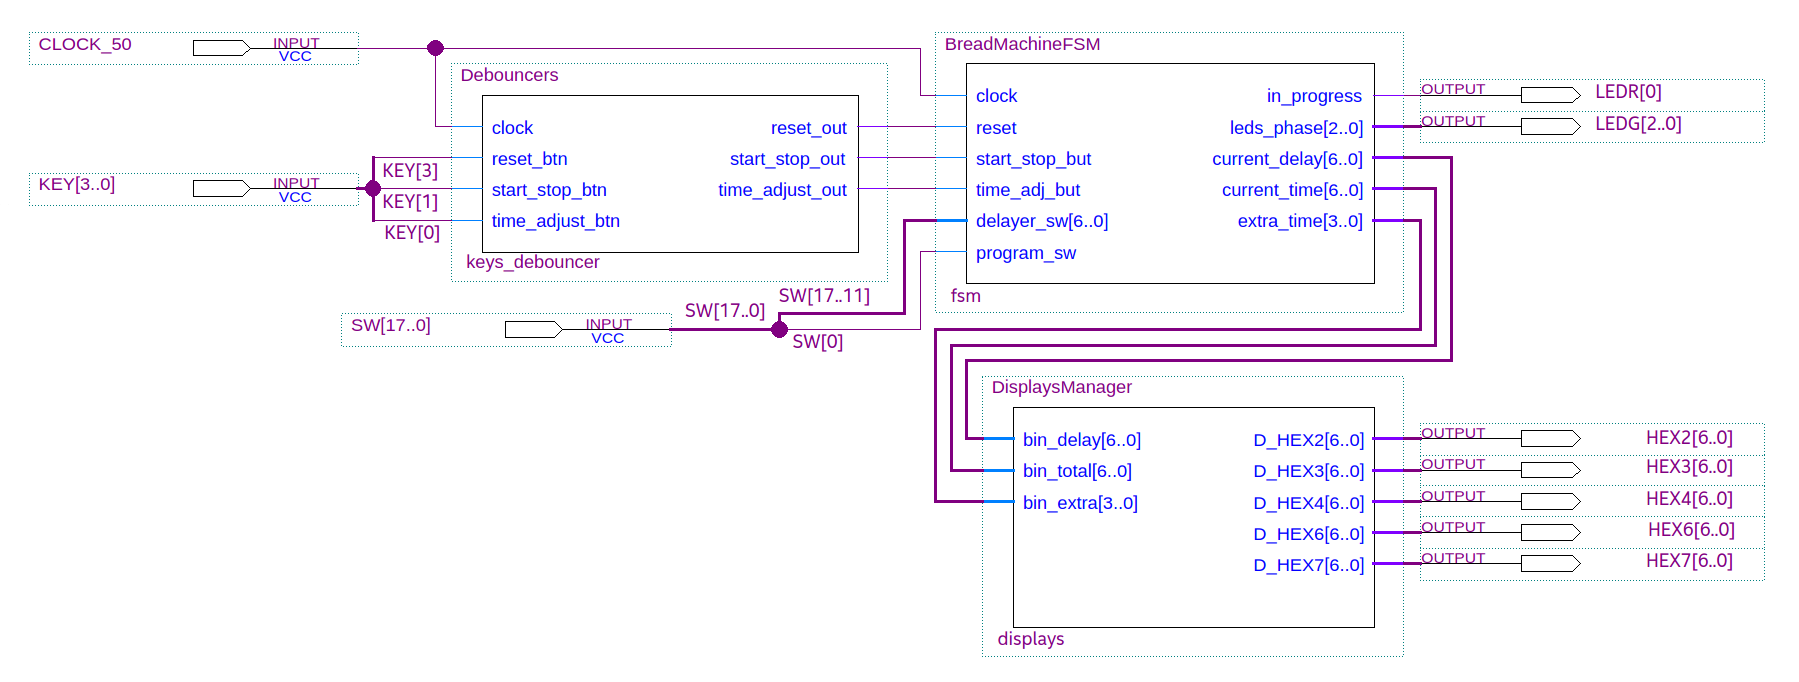
\includegraphics[scale=.25]{../images/top-level-design}\caption{Ilustração do Top-Level da Máquina}
    \label{fig:top-level}
\end{figure}

\section{Debouncers}
\label{sec:debouncers}
Este componente é responsável por fazer o Debounce dos botões.\ Isto é necessário pois quando um botão é pressionado gera centenas de sinais, o que pode muitas vezes causar problemas.

O bloco recebe o valor do relógio geral da máquina bem como os valores dos botões a ser afetados.

Dentro do bloco os valores dos botões são distribuídos entre 3 debouncers onde são processados para gerar os sinais pretendidos.

Sai deste bloco os sinais dos botões já corrigidos para que seja emitido apenas 1 sinal positivo por clique.

\section{BreadMachineFSM}
\label{sec:fsm}
Este é o componente principal da máquina e é o responsável pelo processamento do funcionamento da mesma.

Entram neste componente o sinal do relógio da máquina, os sinais dos botões de `Reiniciar', `Start/Stop' e `Tempo Extra', recebe também o sinal do interruptor do `Selecionador Programa' e, por último, o valor do vetor gerado pelos interruptores do `Selecionador Atraso'.

Como saídas irá ter o sinal para indicar se a máquina se encontra no estado `Progress' ou `Extra'.\ Faz também parte das saídas o vetor de indicação da `Fase da Fabricação' que está a decorrer no momento.\ Estas saídas são diretamente ligadas aos LEDS da máquina: 1 LED vermelho e 3 LEDS verdes, respetivamente.

O funcionamento da máquina de estados será descrito com recurso à figura~\ref{fig:state-machine}.

\pagebreak

\begin{figure}
    \centering
    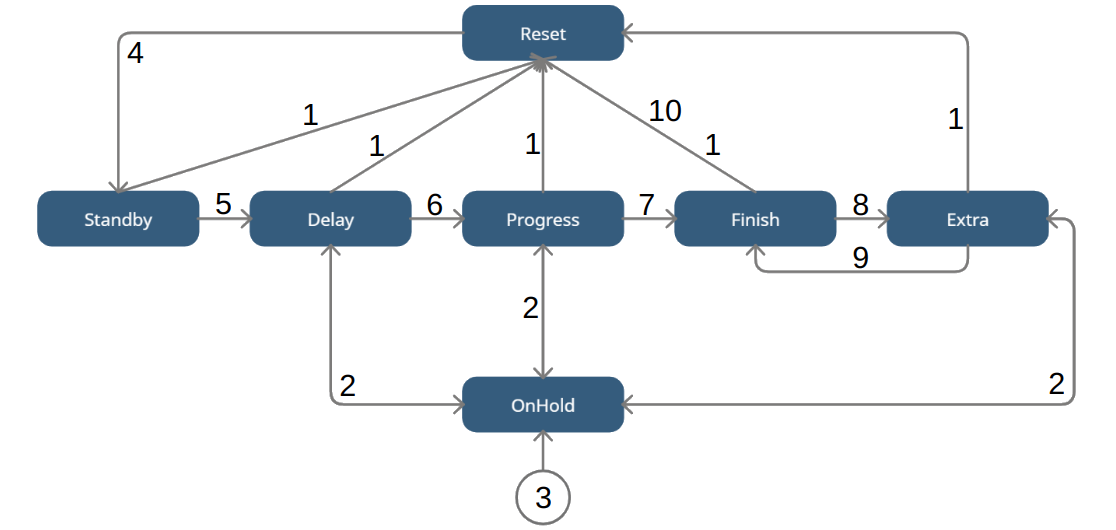
\includegraphics[scale=.4]{../images/state-machine}
    \caption{Esquema da Máquina de Estados}
    \label{fig:state-machine}
\end{figure}

\begin{enumerate}
    \item \textbf{Reset}
        \\$\hookrightarrow$ A máquina volta sempre ao estado de Reset quando o botão `Reset' é pressionado.
    \item \textbf{(Delay/Progress/Extra) $\leftrightarrow$ OnHold}
        \\$\hookrightarrow$ Quando o botão de `Start/Stop' é utilizado e o estado é `Delay', `Progress' ou `Extra', muda o estado para `OnHold' para pausar a máquina.
        \\$\hookrightarrow$ Quando o botão de `Start/Stop' é utilizado e o estado atual é `OnHold', retoma o estado para o qual a máquina se previamente encontrava (`Delay', `Progress' ou `Extra').
    \item \textbf{OnHold $\rightarrow$ OnHold}
        \\$\hookrightarrow$ Atualiza o valor do start\_stop negando o mesmo.\ Fica neste estado enquanto o valor do start\_stop for `0' e sai do estado quando passar para `1'.
    \item \textbf{Reset $\rightarrow$ Standby}
        \\$\hookrightarrow$ Assim que a máquina é reiniciada, o estado muda automaticamente para Standby após a reinicialização de todos os valores.
    \item \textbf{Standby $\rightarrow$ Delay}
        \\$\hookrightarrow$ Quando o botão de `Start/Stop' é pressionado, muda de estado para `Delay' começando o timer do atraso inicial com o valor escolhido.
    \item \textbf{Delay $\rightarrow$ Progress}
        \\$\hookrightarrow$ Assim que o tempo do atraso inicial chegar a 0, o estado passa automaticamente de `Delay' para `Progress'.
    \item \textbf{Progress $\rightarrow$ Finish}
        \\$\hookrightarrow$ Assim que o tempo da programação chegar a 0, o estado passa automaticamente de `Progress' para `Finish'.
        \\$\hookrightarrow$ Neste estado, a máquina não se encontra com nenhuma mudança visual imediata, fica a aguardar por um dos botões.\ Usando o botão `Tempo Extra' poderá ser definido o tempo extra a aplicar à máquina posteriormente no estado `Extra'.
    \item \textbf{Finish $\rightarrow$ Extra}
        \\$\hookrightarrow$ Esta mudança é realizada quando o botão `Start/Stop' é pressionado e o tempo extra não se encontra a 0.
    \item \textbf{Extra $\rightarrow$ Finish}
        \\$\hookrightarrow$ Assim que o tempo do tempo extra chegar a 0, o estado passa automaticamente de `Extra' para `Finish'.
    \item \textbf{Finish $\rightarrow$ Reset}
        \\$\hookrightarrow$ Esta mudança é realizada quando o botão `Start/Stop' é pressionado e o tempo extra encontra-se a 0.\ Este passo reinicializa a máquina automaticamente.
\end{enumerate}

\textbf{Nota:} Os passos 2, 3, 8 e 9 podem ocorrer um número de vezes indefinido durante uma execução completa da máquina.

\section{DisplaysManager}
\label{sec:displays-manager}
Este último componente é o responsável pela gestão dos displays para que os números dos tempos da máquina sejam corretamente visualizados.

O bloco recebe separadamente os valores dos 3 tempos: `Atraso Inicial', `Tempo Normal' e `Tempo Extra'.

O tempo extra é diretamente processado para a codificação dos displays, enquanto que o atraso inicial e o tempo normal têm de ser convertidos em numeração decimal (gerando 2 valores cada) para depois serem codificados.\ Este passo produz 5 valores diferentes.

Esses 5 valores são então distribuídos pelos 5 displays da máquina.